\documentclass[11pt]{article}

    \usepackage[breakable]{tcolorbox}
    \usepackage{parskip} % Stop auto-indenting (to mimic markdown behaviour)
    
    \usepackage{iftex}
    \ifPDFTeX
    	\usepackage[T1]{fontenc}
    	\usepackage{mathpazo}
    \else
    	\usepackage{fontspec}
    \fi

    % Basic figure setup, for now with no caption control since it's done
    % automatically by Pandoc (which extracts ![](path) syntax from Markdown).
    \usepackage{graphicx}
    % Maintain compatibility with old templates. Remove in nbconvert 6.0
    \let\Oldincludegraphics\includegraphics
    % Ensure that by default, figures have no caption (until we provide a
    % proper Figure object with a Caption API and a way to capture that
    % in the conversion process - todo).
    \usepackage{caption}
    \DeclareCaptionFormat{nocaption}{}
    \captionsetup{format=nocaption,aboveskip=0pt,belowskip=0pt}

    \usepackage{float}
    \floatplacement{figure}{H} % forces figures to be placed at the correct location
    \usepackage{xcolor} % Allow colors to be defined
    \usepackage{enumerate} % Needed for markdown enumerations to work
    \usepackage{geometry} % Used to adjust the document margins
    \usepackage{amsmath} % Equations
    \usepackage{amssymb} % Equations
    \usepackage{physics}
    \usepackage{textcomp} % defines textquotesingle
    % Hack from http://tex.stackexchange.com/a/47451/13684:
    \AtBeginDocument{%
        \def\PYZsq{\textquotesingle}% Upright quotes in Pygmentized code
    }
    \usepackage{upquote} % Upright quotes for verbatim code
    \usepackage{eurosym} % defines \euro
    \usepackage[mathletters]{ucs} % Extended unicode (utf-8) support
    \usepackage{fancyvrb} % verbatim replacement that allows latex
    \usepackage{grffile} % extends the file name processing of package graphics 
                         % to support a larger range
    \makeatletter % fix for old versions of grffile with XeLaTeX
    \@ifpackagelater{grffile}{2019/11/01}
    {
      % Do nothing on new versions
    }
    {
      \def\Gread@@xetex#1{%
        \IfFileExists{"\Gin@base".bb}%
        {\Gread@eps{\Gin@base.bb}}%
        {\Gread@@xetex@aux#1}%
      }
    }
    \makeatother
    \usepackage[Export]{adjustbox} % Used to constrain images to a maximum size
    \adjustboxset{max size={0.9\linewidth}{0.9\paperheight}}

    % The hyperref package gives us a pdf with properly built
    % internal navigation ('pdf bookmarks' for the table of contents,
    % internal cross-reference links, web links for URLs, etc.)
    \usepackage{hyperref}
    % The default LaTeX title has an obnoxious amount of whitespace. By default,
    % titling removes some of it. It also provides customization options.
    \usepackage{titling}
    \usepackage{longtable} % longtable support required by pandoc >1.10
    \usepackage{booktabs}  % table support for pandoc > 1.12.2
    \usepackage[inline]{enumitem} % IRkernel/repr support (it uses the enumerate* environment)
    \usepackage[normalem]{ulem} % ulem is needed to support strikethroughs (\sout)
                                % normalem makes italics be italics, not underlines
    \usepackage{mathrsfs}
    

    
    % Colors for the hyperref package
    \definecolor{urlcolor}{rgb}{0,.145,.698}
    \definecolor{linkcolor}{rgb}{.71,0.21,0.01}
    \definecolor{citecolor}{rgb}{.12,.54,.11}

    % ANSI colors
    \definecolor{ansi-black}{HTML}{3E424D}
    \definecolor{ansi-black-intense}{HTML}{282C36}
    \definecolor{ansi-red}{HTML}{E75C58}
    \definecolor{ansi-red-intense}{HTML}{B22B31}
    \definecolor{ansi-green}{HTML}{00A250}
    \definecolor{ansi-green-intense}{HTML}{007427}
    \definecolor{ansi-yellow}{HTML}{DDB62B}
    \definecolor{ansi-yellow-intense}{HTML}{B27D12}
    \definecolor{ansi-blue}{HTML}{208FFB}
    \definecolor{ansi-blue-intense}{HTML}{0065CA}
    \definecolor{ansi-magenta}{HTML}{D160C4}
    \definecolor{ansi-magenta-intense}{HTML}{A03196}
    \definecolor{ansi-cyan}{HTML}{60C6C8}
    \definecolor{ansi-cyan-intense}{HTML}{258F8F}
    \definecolor{ansi-white}{HTML}{C5C1B4}
    \definecolor{ansi-white-intense}{HTML}{A1A6B2}
    \definecolor{ansi-default-inverse-fg}{HTML}{FFFFFF}
    \definecolor{ansi-default-inverse-bg}{HTML}{000000}

    % common color for the border for error outputs.
    \definecolor{outerrorbackground}{HTML}{FFDFDF}

    % commands and environments needed by pandoc snippets
    % extracted from the output of `pandoc -s`
    \providecommand{\tightlist}{%
      \setlength{\itemsep}{0pt}\setlength{\parskip}{0pt}}
    \DefineVerbatimEnvironment{Highlighting}{Verbatim}{commandchars=\\\{\}}
    % Add ',fontsize=\small' for more characters per line
    \newenvironment{Shaded}{}{}
    \newcommand{\KeywordTok}[1]{\textcolor[rgb]{0.00,0.44,0.13}{\textbf{{#1}}}}
    \newcommand{\DataTypeTok}[1]{\textcolor[rgb]{0.56,0.13,0.00}{{#1}}}
    \newcommand{\DecValTok}[1]{\textcolor[rgb]{0.25,0.63,0.44}{{#1}}}
    \newcommand{\BaseNTok}[1]{\textcolor[rgb]{0.25,0.63,0.44}{{#1}}}
    \newcommand{\FloatTok}[1]{\textcolor[rgb]{0.25,0.63,0.44}{{#1}}}
    \newcommand{\CharTok}[1]{\textcolor[rgb]{0.25,0.44,0.63}{{#1}}}
    \newcommand{\StringTok}[1]{\textcolor[rgb]{0.25,0.44,0.63}{{#1}}}
    \newcommand{\CommentTok}[1]{\textcolor[rgb]{0.38,0.63,0.69}{\textit{{#1}}}}
    \newcommand{\OtherTok}[1]{\textcolor[rgb]{0.00,0.44,0.13}{{#1}}}
    \newcommand{\AlertTok}[1]{\textcolor[rgb]{1.00,0.00,0.00}{\textbf{{#1}}}}
    \newcommand{\FunctionTok}[1]{\textcolor[rgb]{0.02,0.16,0.49}{{#1}}}
    \newcommand{\RegionMarkerTok}[1]{{#1}}
    \newcommand{\ErrorTok}[1]{\textcolor[rgb]{1.00,0.00,0.00}{\textbf{{#1}}}}
    \newcommand{\NormalTok}[1]{{#1}}
    
    % Additional commands for more recent versions of Pandoc
    \newcommand{\ConstantTok}[1]{\textcolor[rgb]{0.53,0.00,0.00}{{#1}}}
    \newcommand{\SpecialCharTok}[1]{\textcolor[rgb]{0.25,0.44,0.63}{{#1}}}
    \newcommand{\VerbatimStringTok}[1]{\textcolor[rgb]{0.25,0.44,0.63}{{#1}}}
    \newcommand{\SpecialStringTok}[1]{\textcolor[rgb]{0.73,0.40,0.53}{{#1}}}
    \newcommand{\ImportTok}[1]{{#1}}
    \newcommand{\DocumentationTok}[1]{\textcolor[rgb]{0.73,0.13,0.13}{\textit{{#1}}}}
    \newcommand{\AnnotationTok}[1]{\textcolor[rgb]{0.38,0.63,0.69}{\textbf{\textit{{#1}}}}}
    \newcommand{\CommentVarTok}[1]{\textcolor[rgb]{0.38,0.63,0.69}{\textbf{\textit{{#1}}}}}
    \newcommand{\VariableTok}[1]{\textcolor[rgb]{0.10,0.09,0.49}{{#1}}}
    \newcommand{\ControlFlowTok}[1]{\textcolor[rgb]{0.00,0.44,0.13}{\textbf{{#1}}}}
    \newcommand{\OperatorTok}[1]{\textcolor[rgb]{0.40,0.40,0.40}{{#1}}}
    \newcommand{\BuiltInTok}[1]{{#1}}
    \newcommand{\ExtensionTok}[1]{{#1}}
    \newcommand{\PreprocessorTok}[1]{\textcolor[rgb]{0.74,0.48,0.00}{{#1}}}
    \newcommand{\AttributeTok}[1]{\textcolor[rgb]{0.49,0.56,0.16}{{#1}}}
    \newcommand{\InformationTok}[1]{\textcolor[rgb]{0.38,0.63,0.69}{\textbf{\textit{{#1}}}}}
    \newcommand{\WarningTok}[1]{\textcolor[rgb]{0.38,0.63,0.69}{\textbf{\textit{{#1}}}}}
    
    
    % Define a nice break command that doesn't care if a line doesn't already
    % exist.
    \def\br{\hspace*{\fill} \\* }
    % Math Jax compatibility definitions
    \def\gt{>}
    \def\lt{<}
    \let\Oldtex\TeX
    \let\Oldlatex\LaTeX
    \renewcommand{\TeX}{\textrm{\Oldtex}}
    \renewcommand{\LaTeX}{\textrm{\Oldlatex}}
    % Document parameters
    % Document title
    \title{PC3233 Assignment 4}
    
    
    
    
    
% Pygments definitions
\makeatletter
\def\PY@reset{\let\PY@it=\relax \let\PY@bf=\relax%
    \let\PY@ul=\relax \let\PY@tc=\relax%
    \let\PY@bc=\relax \let\PY@ff=\relax}
\def\PY@tok#1{\csname PY@tok@#1\endcsname}
\def\PY@toks#1+{\ifx\relax#1\empty\else%
    \PY@tok{#1}\expandafter\PY@toks\fi}
\def\PY@do#1{\PY@bc{\PY@tc{\PY@ul{%
    \PY@it{\PY@bf{\PY@ff{#1}}}}}}}
\def\PY#1#2{\PY@reset\PY@toks#1+\relax+\PY@do{#2}}

\@namedef{PY@tok@w}{\def\PY@tc##1{\textcolor[rgb]{0.73,0.73,0.73}{##1}}}
\@namedef{PY@tok@c}{\let\PY@it=\textit\def\PY@tc##1{\textcolor[rgb]{0.24,0.48,0.48}{##1}}}
\@namedef{PY@tok@cp}{\def\PY@tc##1{\textcolor[rgb]{0.61,0.40,0.00}{##1}}}
\@namedef{PY@tok@k}{\let\PY@bf=\textbf\def\PY@tc##1{\textcolor[rgb]{0.00,0.50,0.00}{##1}}}
\@namedef{PY@tok@kp}{\def\PY@tc##1{\textcolor[rgb]{0.00,0.50,0.00}{##1}}}
\@namedef{PY@tok@kt}{\def\PY@tc##1{\textcolor[rgb]{0.69,0.00,0.25}{##1}}}
\@namedef{PY@tok@o}{\def\PY@tc##1{\textcolor[rgb]{0.40,0.40,0.40}{##1}}}
\@namedef{PY@tok@ow}{\let\PY@bf=\textbf\def\PY@tc##1{\textcolor[rgb]{0.67,0.13,1.00}{##1}}}
\@namedef{PY@tok@nb}{\def\PY@tc##1{\textcolor[rgb]{0.00,0.50,0.00}{##1}}}
\@namedef{PY@tok@nf}{\def\PY@tc##1{\textcolor[rgb]{0.00,0.00,1.00}{##1}}}
\@namedef{PY@tok@nc}{\let\PY@bf=\textbf\def\PY@tc##1{\textcolor[rgb]{0.00,0.00,1.00}{##1}}}
\@namedef{PY@tok@nn}{\let\PY@bf=\textbf\def\PY@tc##1{\textcolor[rgb]{0.00,0.00,1.00}{##1}}}
\@namedef{PY@tok@ne}{\let\PY@bf=\textbf\def\PY@tc##1{\textcolor[rgb]{0.80,0.25,0.22}{##1}}}
\@namedef{PY@tok@nv}{\def\PY@tc##1{\textcolor[rgb]{0.10,0.09,0.49}{##1}}}
\@namedef{PY@tok@no}{\def\PY@tc##1{\textcolor[rgb]{0.53,0.00,0.00}{##1}}}
\@namedef{PY@tok@nl}{\def\PY@tc##1{\textcolor[rgb]{0.46,0.46,0.00}{##1}}}
\@namedef{PY@tok@ni}{\let\PY@bf=\textbf\def\PY@tc##1{\textcolor[rgb]{0.44,0.44,0.44}{##1}}}
\@namedef{PY@tok@na}{\def\PY@tc##1{\textcolor[rgb]{0.41,0.47,0.13}{##1}}}
\@namedef{PY@tok@nt}{\let\PY@bf=\textbf\def\PY@tc##1{\textcolor[rgb]{0.00,0.50,0.00}{##1}}}
\@namedef{PY@tok@nd}{\def\PY@tc##1{\textcolor[rgb]{0.67,0.13,1.00}{##1}}}
\@namedef{PY@tok@s}{\def\PY@tc##1{\textcolor[rgb]{0.73,0.13,0.13}{##1}}}
\@namedef{PY@tok@sd}{\let\PY@it=\textit\def\PY@tc##1{\textcolor[rgb]{0.73,0.13,0.13}{##1}}}
\@namedef{PY@tok@si}{\let\PY@bf=\textbf\def\PY@tc##1{\textcolor[rgb]{0.64,0.35,0.47}{##1}}}
\@namedef{PY@tok@se}{\let\PY@bf=\textbf\def\PY@tc##1{\textcolor[rgb]{0.67,0.36,0.12}{##1}}}
\@namedef{PY@tok@sr}{\def\PY@tc##1{\textcolor[rgb]{0.64,0.35,0.47}{##1}}}
\@namedef{PY@tok@ss}{\def\PY@tc##1{\textcolor[rgb]{0.10,0.09,0.49}{##1}}}
\@namedef{PY@tok@sx}{\def\PY@tc##1{\textcolor[rgb]{0.00,0.50,0.00}{##1}}}
\@namedef{PY@tok@m}{\def\PY@tc##1{\textcolor[rgb]{0.40,0.40,0.40}{##1}}}
\@namedef{PY@tok@gh}{\let\PY@bf=\textbf\def\PY@tc##1{\textcolor[rgb]{0.00,0.00,0.50}{##1}}}
\@namedef{PY@tok@gu}{\let\PY@bf=\textbf\def\PY@tc##1{\textcolor[rgb]{0.50,0.00,0.50}{##1}}}
\@namedef{PY@tok@gd}{\def\PY@tc##1{\textcolor[rgb]{0.63,0.00,0.00}{##1}}}
\@namedef{PY@tok@gi}{\def\PY@tc##1{\textcolor[rgb]{0.00,0.52,0.00}{##1}}}
\@namedef{PY@tok@gr}{\def\PY@tc##1{\textcolor[rgb]{0.89,0.00,0.00}{##1}}}
\@namedef{PY@tok@ge}{\let\PY@it=\textit}
\@namedef{PY@tok@gs}{\let\PY@bf=\textbf}
\@namedef{PY@tok@gp}{\let\PY@bf=\textbf\def\PY@tc##1{\textcolor[rgb]{0.00,0.00,0.50}{##1}}}
\@namedef{PY@tok@go}{\def\PY@tc##1{\textcolor[rgb]{0.44,0.44,0.44}{##1}}}
\@namedef{PY@tok@gt}{\def\PY@tc##1{\textcolor[rgb]{0.00,0.27,0.87}{##1}}}
\@namedef{PY@tok@err}{\def\PY@bc##1{{\setlength{\fboxsep}{\string -\fboxrule}\fcolorbox[rgb]{1.00,0.00,0.00}{1,1,1}{\strut ##1}}}}
\@namedef{PY@tok@kc}{\let\PY@bf=\textbf\def\PY@tc##1{\textcolor[rgb]{0.00,0.50,0.00}{##1}}}
\@namedef{PY@tok@kd}{\let\PY@bf=\textbf\def\PY@tc##1{\textcolor[rgb]{0.00,0.50,0.00}{##1}}}
\@namedef{PY@tok@kn}{\let\PY@bf=\textbf\def\PY@tc##1{\textcolor[rgb]{0.00,0.50,0.00}{##1}}}
\@namedef{PY@tok@kr}{\let\PY@bf=\textbf\def\PY@tc##1{\textcolor[rgb]{0.00,0.50,0.00}{##1}}}
\@namedef{PY@tok@bp}{\def\PY@tc##1{\textcolor[rgb]{0.00,0.50,0.00}{##1}}}
\@namedef{PY@tok@fm}{\def\PY@tc##1{\textcolor[rgb]{0.00,0.00,1.00}{##1}}}
\@namedef{PY@tok@vc}{\def\PY@tc##1{\textcolor[rgb]{0.10,0.09,0.49}{##1}}}
\@namedef{PY@tok@vg}{\def\PY@tc##1{\textcolor[rgb]{0.10,0.09,0.49}{##1}}}
\@namedef{PY@tok@vi}{\def\PY@tc##1{\textcolor[rgb]{0.10,0.09,0.49}{##1}}}
\@namedef{PY@tok@vm}{\def\PY@tc##1{\textcolor[rgb]{0.10,0.09,0.49}{##1}}}
\@namedef{PY@tok@sa}{\def\PY@tc##1{\textcolor[rgb]{0.73,0.13,0.13}{##1}}}
\@namedef{PY@tok@sb}{\def\PY@tc##1{\textcolor[rgb]{0.73,0.13,0.13}{##1}}}
\@namedef{PY@tok@sc}{\def\PY@tc##1{\textcolor[rgb]{0.73,0.13,0.13}{##1}}}
\@namedef{PY@tok@dl}{\def\PY@tc##1{\textcolor[rgb]{0.73,0.13,0.13}{##1}}}
\@namedef{PY@tok@s2}{\def\PY@tc##1{\textcolor[rgb]{0.73,0.13,0.13}{##1}}}
\@namedef{PY@tok@sh}{\def\PY@tc##1{\textcolor[rgb]{0.73,0.13,0.13}{##1}}}
\@namedef{PY@tok@s1}{\def\PY@tc##1{\textcolor[rgb]{0.73,0.13,0.13}{##1}}}
\@namedef{PY@tok@mb}{\def\PY@tc##1{\textcolor[rgb]{0.40,0.40,0.40}{##1}}}
\@namedef{PY@tok@mf}{\def\PY@tc##1{\textcolor[rgb]{0.40,0.40,0.40}{##1}}}
\@namedef{PY@tok@mh}{\def\PY@tc##1{\textcolor[rgb]{0.40,0.40,0.40}{##1}}}
\@namedef{PY@tok@mi}{\def\PY@tc##1{\textcolor[rgb]{0.40,0.40,0.40}{##1}}}
\@namedef{PY@tok@il}{\def\PY@tc##1{\textcolor[rgb]{0.40,0.40,0.40}{##1}}}
\@namedef{PY@tok@mo}{\def\PY@tc##1{\textcolor[rgb]{0.40,0.40,0.40}{##1}}}
\@namedef{PY@tok@ch}{\let\PY@it=\textit\def\PY@tc##1{\textcolor[rgb]{0.24,0.48,0.48}{##1}}}
\@namedef{PY@tok@cm}{\let\PY@it=\textit\def\PY@tc##1{\textcolor[rgb]{0.24,0.48,0.48}{##1}}}
\@namedef{PY@tok@cpf}{\let\PY@it=\textit\def\PY@tc##1{\textcolor[rgb]{0.24,0.48,0.48}{##1}}}
\@namedef{PY@tok@c1}{\let\PY@it=\textit\def\PY@tc##1{\textcolor[rgb]{0.24,0.48,0.48}{##1}}}
\@namedef{PY@tok@cs}{\let\PY@it=\textit\def\PY@tc##1{\textcolor[rgb]{0.24,0.48,0.48}{##1}}}

\def\PYZbs{\char`\\}
\def\PYZus{\char`\_}
\def\PYZob{\char`\{}
\def\PYZcb{\char`\}}
\def\PYZca{\char`\^}
\def\PYZam{\char`\&}
\def\PYZlt{\char`\<}
\def\PYZgt{\char`\>}
\def\PYZsh{\char`\#}
\def\PYZpc{\char`\%}
\def\PYZdl{\char`\$}
\def\PYZhy{\char`\-}
\def\PYZsq{\char`\'}
\def\PYZdq{\char`\"}
\def\PYZti{\char`\~}
% for compatibility with earlier versions
\def\PYZat{@}
\def\PYZlb{[}
\def\PYZrb{]}
\makeatother


    % For linebreaks inside Verbatim environment from package fancyvrb. 
    \makeatletter
        \newbox\Wrappedcontinuationbox 
        \newbox\Wrappedvisiblespacebox 
        \newcommand*\Wrappedvisiblespace {\textcolor{red}{\textvisiblespace}} 
        \newcommand*\Wrappedcontinuationsymbol {\textcolor{red}{\llap{\tiny$\m@th\hookrightarrow$}}} 
        \newcommand*\Wrappedcontinuationindent {3ex } 
        \newcommand*\Wrappedafterbreak {\kern\Wrappedcontinuationindent\copy\Wrappedcontinuationbox} 
        % Take advantage of the already applied Pygments mark-up to insert 
        % potential linebreaks for TeX processing. 
        %        {, <, #, %, $, ' and ": go to next line. 
        %        _, }, ^, &, >, - and ~: stay at end of broken line. 
        % Use of \textquotesingle for straight quote. 
        \newcommand*\Wrappedbreaksatspecials {% 
            \def\PYGZus{\discretionary{\char`\_}{\Wrappedafterbreak}{\char`\_}}% 
            \def\PYGZob{\discretionary{}{\Wrappedafterbreak\char`\{}{\char`\{}}% 
            \def\PYGZcb{\discretionary{\char`\}}{\Wrappedafterbreak}{\char`\}}}% 
            \def\PYGZca{\discretionary{\char`\^}{\Wrappedafterbreak}{\char`\^}}% 
            \def\PYGZam{\discretionary{\char`\&}{\Wrappedafterbreak}{\char`\&}}% 
            \def\PYGZlt{\discretionary{}{\Wrappedafterbreak\char`\<}{\char`\<}}% 
            \def\PYGZgt{\discretionary{\char`\>}{\Wrappedafterbreak}{\char`\>}}% 
            \def\PYGZsh{\discretionary{}{\Wrappedafterbreak\char`\#}{\char`\#}}% 
            \def\PYGZpc{\discretionary{}{\Wrappedafterbreak\char`\%}{\char`\%}}% 
            \def\PYGZdl{\discretionary{}{\Wrappedafterbreak\char`\$}{\char`\$}}% 
            \def\PYGZhy{\discretionary{\char`\-}{\Wrappedafterbreak}{\char`\-}}% 
            \def\PYGZsq{\discretionary{}{\Wrappedafterbreak\textquotesingle}{\textquotesingle}}% 
            \def\PYGZdq{\discretionary{}{\Wrappedafterbreak\char`\"}{\char`\"}}% 
            \def\PYGZti{\discretionary{\char`\~}{\Wrappedafterbreak}{\char`\~}}% 
        } 
        % Some characters . , ; ? ! / are not pygmentized. 
        % This macro makes them "active" and they will insert potential linebreaks 
        \newcommand*\Wrappedbreaksatpunct {% 
            \lccode`\~`\.\lowercase{\def~}{\discretionary{\hbox{\char`\.}}{\Wrappedafterbreak}{\hbox{\char`\.}}}% 
            \lccode`\~`\,\lowercase{\def~}{\discretionary{\hbox{\char`\,}}{\Wrappedafterbreak}{\hbox{\char`\,}}}% 
            \lccode`\~`\;\lowercase{\def~}{\discretionary{\hbox{\char`\;}}{\Wrappedafterbreak}{\hbox{\char`\;}}}% 
            \lccode`\~`\:\lowercase{\def~}{\discretionary{\hbox{\char`\:}}{\Wrappedafterbreak}{\hbox{\char`\:}}}% 
            \lccode`\~`\?\lowercase{\def~}{\discretionary{\hbox{\char`\?}}{\Wrappedafterbreak}{\hbox{\char`\?}}}% 
            \lccode`\~`\!\lowercase{\def~}{\discretionary{\hbox{\char`\!}}{\Wrappedafterbreak}{\hbox{\char`\!}}}% 
            \lccode`\~`\/\lowercase{\def~}{\discretionary{\hbox{\char`\/}}{\Wrappedafterbreak}{\hbox{\char`\/}}}% 
            \catcode`\.\active
            \catcode`\,\active 
            \catcode`\;\active
            \catcode`\:\active
            \catcode`\?\active
            \catcode`\!\active
            \catcode`\/\active 
            \lccode`\~`\~ 	
        }
    \makeatother

    \let\OriginalVerbatim=\Verbatim
    \makeatletter
    \renewcommand{\Verbatim}[1][1]{%
        %\parskip\z@skip
        \sbox\Wrappedcontinuationbox {\Wrappedcontinuationsymbol}%
        \sbox\Wrappedvisiblespacebox {\FV@SetupFont\Wrappedvisiblespace}%
        \def\FancyVerbFormatLine ##1{\hsize\linewidth
            \vtop{\raggedright\hyphenpenalty\z@\exhyphenpenalty\z@
                \doublehyphendemerits\z@\finalhyphendemerits\z@
                \strut ##1\strut}%
        }%
        % If the linebreak is at a space, the latter will be displayed as visible
        % space at end of first line, and a continuation symbol starts next line.
        % Stretch/shrink are however usually zero for typewriter font.
        \def\FV@Space {%
            \nobreak\hskip\z@ plus\fontdimen3\font minus\fontdimen4\font
            \discretionary{\copy\Wrappedvisiblespacebox}{\Wrappedafterbreak}
            {\kern\fontdimen2\font}%
        }%
        
        % Allow breaks at special characters using \PYG... macros.
        \Wrappedbreaksatspecials
        % Breaks at punctuation characters . , ; ? ! and / need catcode=\active 	
        \OriginalVerbatim[#1,codes*=\Wrappedbreaksatpunct]%
    }
    \makeatother

    % Exact colors from NB
    \definecolor{incolor}{HTML}{303F9F}
    \definecolor{outcolor}{HTML}{D84315}
    \definecolor{cellborder}{HTML}{CFCFCF}
    \definecolor{cellbackground}{HTML}{F7F7F7}
    
    % prompt
    \makeatletter
    \newcommand{\boxspacing}{\kern\kvtcb@left@rule\kern\kvtcb@boxsep}
    \makeatother
    \newcommand{\prompt}[4]{
        {\ttfamily\llap{{\color{#2}[#3]:\hspace{3pt}#4}}\vspace{-\baselineskip}}
    }
    

    
    % Prevent overflowing lines due to hard-to-break entities
    \sloppy 
    % Setup hyperref package
    \hypersetup{
      breaklinks=true,  % so long urls are correctly broken across lines
      colorlinks=true,
      urlcolor=urlcolor,
      linkcolor=linkcolor,
      citecolor=citecolor,
      }
    % Slightly bigger margins than the latex defaults
    
    \geometry{verbose,tmargin=1in,bmargin=1in,lmargin=1in,rmargin=1in}
    
    

\begin{document}
    
    \maketitle
    
    \section{Hydrogen Atom}
    Prove the identity for the Pauli matrices, $\pmb{\sigma}$ and general vector operators $\mathbf{A}$ and $\mathbf{B}$:
    \begin{equation}
    (\pmb{\sigma} \cdot \mathbf{A})  (\pmb{\sigma} \cdot \mathbf{B}) = (\mathbf{A} \cdot \mathbf{B}) + i\pmb{\sigma} \cdot (\mathbf{A} \times \mathbf{B})
    \end{equation}

    \subsection{Proof}
    \begin{equation}
        (\pmb{\sigma} \cdot \mathbf{A})  (\pmb{\sigma} \cdot \mathbf{B}) = \sum_{ij} \sigma_i A_i \sigma_j B_j
    \end{equation}
    Since $\commutator{\sigma_i}{\sigma_j} = \sigma_i \sigma_j - \sigma_j \sigma_i$, we can expand the above expression as:
    \begin{equation}
        \sum_{ij} \sigma_i A_i \sigma_j B_j = \sum_{ij} (\commutator{\sigma_i}{\sigma_j} + \sigma_j \sigma_i) A_i B_j
    \end{equation}
    Using the anticommutation property of the Pauli matrices, $\anticommutator{\sigma_i}{\sigma_j} = \sigma_i \sigma_j + \sigma_j \sigma_i$ we have:
    \begin{align*}
        \sum_{ij} (\commutator{\sigma_i}{\sigma_j} + \sigma_j \sigma_i) A_i B_j 
        &= \sum_{ij}( 2 i \epsilon_{ijk} \sigma_k A_i B_j + (\anticommutator{\sigma_i}{\sigma_j} - \sigma_i \sigma_j) A_i B_j) \\
        &= \sum_{ij} (2 i \sigma_k (\mathbf{A} \times \mathbf{B})_k + 2 \delta_{ij} A_i B_j - \sigma_i A_i \sigma_j B_j) \\
        &= 2 i \pmb{\sigma} \cdot (\mathbf{A} \times \mathbf{B}) + 2 \mathbf{A} \cdot \mathbf{B} - (\pmb{\sigma} \cdot \mathbf{A}) (\pmb{\sigma} \cdot \mathbf{B}) \\
    \end{align*}
    Rearranging the terms, we have:
    \begin{align*}
        & (\pmb{\sigma} \cdot \mathbf{A})  (\pmb{\sigma} \cdot \mathbf{B}) = 2 i \pmb{\sigma} \cdot (\mathbf{A} \times \mathbf{B}) + 2 \mathbf{A} \cdot \mathbf{B} - (\pmb{\sigma} \cdot \mathbf{A}) (\pmb{\sigma} \cdot \mathbf{B}) \\
        & 2 (\pmb{\sigma} \cdot \mathbf{A})  (\pmb{\sigma} \cdot \mathbf{B}) = 2 i \pmb{\sigma} \cdot (\mathbf{A} \times \mathbf{B}) + 2 \mathbf{A} \cdot \mathbf{B} \\
        & (\pmb{\sigma} \cdot \mathbf{A})  (\pmb{\sigma} \cdot \mathbf{B}) = (\mathbf{A} \cdot \mathbf{B}) + i\pmb{\sigma} \cdot (\mathbf{A} \times \mathbf{B})
    \end{align*}
    Hence, we have proved the identity.

    \newpage
    \section{Fine Structure}

    \subsection{Determine the frequencies of absorption lines from 1S to 2P and 2P for (1H, 2D, 3T)}

    The reduced mass is given by:
    \begin{equation}
        \begin{cases}
            \mu_H = \frac{m_N m_e}{m_N + m_e} = 9.1044 \times 10^{-31} & \text{for Hydrogen, $m_N = m_p$} \\
            \mu_D = \frac{m_N m_e}{m_N + m_e} = 9.1069 \times 10^{-31} & \text{for Deuterium, $m_N = m_p + m_n$} \\
            \mu_T = \frac{m_N m_e}{m_N + m_e} = 9.1077 \times 10^{-31} & \text{for Tritium, $m_N = m_p + 2m_n$}
        \end{cases}
    \end{equation}

    Then we can compute the energy levels of the hydrogen atom using the Bohr model, which is given by:

    \begin{equation}
        E_n = - \frac{\mu e^4 Z^2}{8 \epsilon_0^2 h^2 n^2} 
    \end{equation}

    Therefore, we can get the energy difference between the 1S and 2P states by:

    \begin{equation}
        \Delta E_{1S-2P} = E_1 - E_2
    \end{equation}
    
    where $E_1$ and $E_2$ are the energy levels of the 1S and 2P states respectively. 

    \begin{equation}
        \begin{cases}
            E_{1S-2P} = -2.178686 \times 10^{-18} \text{J} & \text{for Hydrogen} \\
            E_{1S-2P} = -2.179279 \times 10^{-18} \text{J} & \text{for Deuterium} \\
            E_{1S-2P} = -2.179477 \times 10^{-18} \text{J} & \text{for Tritium}
        \end{cases}
    \end{equation}

    By using the Planck relation, $E = h\nu$, we can compute the frequency of the absorption lines:

    \begin{equation}
        \begin{cases}
            \nu_{1S-2P} = \frac{E_{1S-2P}}{h} = 2.466038 \times 10^{15} \text{Hz} & \text{for Hydrogen} \\
            \nu_{1S-2P} = \frac{E_{1S-2P}}{h} = 2.466710 \times 10^{15} \text{Hz} & \text{for Deuterium} \\
            \nu_{1S-2P} = \frac{E_{1S-2P}}{h} = 2.466934 \times 10^{15} \text{Hz} & \text{for Tritium}
        \end{cases}
    \end{equation}

    \subsection{Relativistic Correction}

    The relativistic mass correction to the energy levels of the hydrogen atom is given by:

    \begin{equation}
        \Delta E^m_{rel} = -E_n \frac{Z^2 \alpha^2}{n} (\frac{3}{4n} - \frac{1}{l + \frac{1}{2}})
    \end{equation}

    where $E_n = -13.6 \text{eV}$ is the non-relativistic energy level, $Z = 1$ is the atomic number, $\alpha = \frac{e^2}{\hbar c}$ is the fine structure constant, $n$ is the principal quantum number and $l$ is the azimuthal quantum number.

    \begin{equation}
        \begin{cases}
            \Delta E_{\text{rel}} = -13.6 \, \text{eV} \times \frac{1^2 \alpha^2}{1} \left(\frac{3}{4 \times 1} - \frac{1}{\frac{1}{2}}\right) = -9.05 \times 10^{-4} \, \text{eV} & \text{for 1S} \\
            \Delta E_{\text{rel}} = -13.6 \, \text{eV} \times \frac{1^2 \alpha^2}{2} \left(\frac{3}{4 \times 2} - \frac{1}{1 + \frac{1}{2}}\right) = -2.6 \times 10^{-5} \, \text{eV} & \text{for 2P} \\
        \end{cases}
    \end{equation}

    The Darwin term is given by:

    \begin{equation}
        \begin{cases}
            \Delta E^D_{rel} = -E_n \frac{Z^2 \alpha^2}{n} & \text{for $l = 0$} \\
            \Delta E^D_{rel} = 0 & \text{for $l \neq 0$}
        \end{cases}
    \end{equation}

    Hence, we get:

    \begin{equation}
        \begin{cases}
            \Delta E_{\text{Darwin}} = 7.24 \times 10^{-4} \, \text{eV} & \text{for 1S} \\
            \Delta E_{\text{Darwin}} = 0 & \text{for 2P} \\
        \end{cases}
    \end{equation}
    
    \subsection{Spin-Orbit Coupling}

    The spin-orbit coupling is given by:

    \begin{equation}
        \Delta E_{\text{SO}} = -E_n \frac{Z^2 \alpha^2}{n \cdot l(l+\frac{1}{2})(l+1)}
    \end{equation}

    Therefore, we have:

    \begin{equation}
        \begin{cases}
            \Delta E_{\text{SO}} = 0 & \text{for 1S} \\
            \Delta E_{\text{SO}} = 4.5 \times 10^{-5} \, \text{eV} & \text{for 2P} \\
        \end{cases}
    \end{equation}

    \subsection{Working}
    
\begin{tcolorbox}[breakable, size=fbox, boxrule=1pt, pad at break*=1mm,colback=cellbackground, colframe=cellborder]
\prompt{In}{incolor}{1}{\boxspacing}
\begin{Verbatim}[commandchars=\\\{\}]
\PY{k+kn}{import} \PY{n+nn}{scipy}\PY{n+nn}{.}\PY{n+nn}{constants} \PY{k}{as} \PY{n+nn}{sp}
\PY{k+kn}{import} \PY{n+nn}{pandas} \PY{k}{as} \PY{n+nn}{pd}
\end{Verbatim}
\end{tcolorbox}

    \begin{tcolorbox}[breakable, size=fbox, boxrule=1pt, pad at break*=1mm,colback=cellbackground, colframe=cellborder]
\prompt{In}{incolor}{2}{\boxspacing}
\begin{Verbatim}[commandchars=\\\{\}]
\PY{c+c1}{\PYZsh{} constant}
\PY{n}{m\PYZus{}e} \PY{o}{=} \PY{n}{sp}\PY{o}{.}\PY{n}{electron\PYZus{}mass}
\PY{n}{m\PYZus{}p} \PY{o}{=} \PY{n}{sp}\PY{o}{.}\PY{n}{proton\PYZus{}mass}
\PY{n}{m\PYZus{}n} \PY{o}{=} \PY{n}{sp}\PY{o}{.}\PY{n}{neutron\PYZus{}mass}
\PY{n}{h} \PY{o}{=} \PY{n}{sp}\PY{o}{.}\PY{n}{Planck}
\PY{n}{e\PYZus{}0} \PY{o}{=} \PY{n}{sp}\PY{o}{.}\PY{n}{epsilon\PYZus{}0}
\PY{n}{e} \PY{o}{=} \PY{n}{sp}\PY{o}{.}\PY{n}{e}
\PY{n}{alpha} \PY{o}{=} \PY{n}{sp}\PY{o}{.}\PY{n}{fine\PYZus{}structure}
\end{Verbatim}
\end{tcolorbox}

    \begin{tcolorbox}[breakable, size=fbox, boxrule=1pt, pad at break*=1mm,colback=cellbackground, colframe=cellborder]
\prompt{In}{incolor}{3}{\boxspacing}
\begin{Verbatim}[commandchars=\\\{\}]
\PY{k}{class} \PY{n+nc}{Atom}\PY{p}{:}
    \PY{k}{def} \PY{n+nf+fm}{\PYZus{}\PYZus{}init\PYZus{}\PYZus{}}\PY{p}{(}\PY{n+nb+bp}{self}\PY{p}{,} \PY{n}{proton\PYZus{}num}\PY{p}{,} \PY{n}{nuetron\PYZus{}num}\PY{p}{,} \PY{n}{electron\PYZus{}num}\PY{p}{,} \PY{n}{name}\PY{p}{)}\PY{p}{:}
        \PY{n+nb+bp}{self}\PY{o}{.}\PY{n}{pn} \PY{o}{=} \PY{n}{proton\PYZus{}num}
        \PY{n+nb+bp}{self}\PY{o}{.}\PY{n}{en} \PY{o}{=} \PY{n}{electron\PYZus{}num}
        \PY{n+nb+bp}{self}\PY{o}{.}\PY{n}{nn} \PY{o}{=} \PY{n}{nuetron\PYZus{}num}
        \PY{n+nb+bp}{self}\PY{o}{.}\PY{n}{name} \PY{o}{=} \PY{n}{name}
    
    \PY{k}{def} \PY{n+nf}{compute\PYZus{}reduce\PYZus{}mass}\PY{p}{(}\PY{n+nb+bp}{self}\PY{p}{)}\PY{p}{:}
        \PY{n}{norm} \PY{o}{=} \PY{p}{(}\PY{n+nb+bp}{self}\PY{o}{.}\PY{n}{nn} \PY{o}{*} \PY{n}{m\PYZus{}n} \PY{o}{+} \PY{n+nb+bp}{self}\PY{o}{.}\PY{n}{pn} \PY{o}{*} \PY{n}{m\PYZus{}p}\PY{p}{)} \PY{o}{*} \PY{n+nb+bp}{self}\PY{o}{.}\PY{n}{en} \PY{o}{*} \PY{n}{m\PYZus{}e}
        \PY{n}{denorm} \PY{o}{=} \PY{p}{(}\PY{n+nb+bp}{self}\PY{o}{.}\PY{n}{nn} \PY{o}{*} \PY{n}{m\PYZus{}n} \PY{o}{+} \PY{n+nb+bp}{self}\PY{o}{.}\PY{n}{pn} \PY{o}{*} \PY{n}{m\PYZus{}p}\PY{p}{)} \PY{o}{+} \PY{n+nb+bp}{self}\PY{o}{.}\PY{n}{en} \PY{o}{*} \PY{n}{m\PYZus{}e}
        \PY{k}{return} \PY{n}{norm} \PY{o}{/} \PY{n}{denorm}
    
    \PY{k}{def} \PY{n+nf}{compute\PYZus{}energy\PYZus{}level\PYZus{}in\PYZus{}Joule}\PY{p}{(}\PY{n+nb+bp}{self}\PY{p}{,} \PY{n}{n}\PY{p}{)}\PY{p}{:}
        \PY{n}{mu} \PY{o}{=} \PY{n+nb+bp}{self}\PY{o}{.}\PY{n}{compute\PYZus{}reduce\PYZus{}mass}\PY{p}{(}\PY{p}{)}
        \PY{n}{norm} \PY{o}{=} \PY{n}{mu} \PY{o}{*} \PY{n}{e} \PY{o}{*}\PY{o}{*} \PY{l+m+mi}{4} \PY{o}{*} \PY{n+nb+bp}{self}\PY{o}{.}\PY{n}{pn} \PY{o}{*}\PY{o}{*} \PY{l+m+mi}{2}
        \PY{n}{denorm} \PY{o}{=} \PY{l+m+mi}{8} \PY{o}{*} \PY{n}{e\PYZus{}0}\PY{o}{*}\PY{o}{*}\PY{l+m+mi}{2} \PY{o}{*} \PY{n}{h}\PY{o}{*}\PY{o}{*}\PY{l+m+mi}{2} \PY{o}{*} \PY{n}{n}\PY{o}{*}\PY{o}{*}\PY{l+m+mi}{2}
        \PY{k}{return} \PY{o}{\PYZhy{}} \PY{n}{norm}\PY{o}{/}\PY{n}{denorm}
    
    \PY{k}{def} \PY{n+nf}{compute\PYZus{}energy\PYZus{}level\PYZus{}in\PYZus{}eV}\PY{p}{(}\PY{n+nb+bp}{self}\PY{p}{,} \PY{n}{n}\PY{p}{)}\PY{p}{:}
        \PY{k}{return} \PY{n+nb+bp}{self}\PY{o}{.}\PY{n}{compute\PYZus{}energy\PYZus{}level\PYZus{}in\PYZus{}Joule}\PY{p}{(}\PY{n}{n}\PY{p}{)} \PY{o}{/} \PY{n}{e}
    
    \PY{k}{def} \PY{n+nf}{determine\PYZus{}frequency}\PY{p}{(}\PY{n+nb+bp}{self}\PY{p}{,} \PY{n}{n1}\PY{p}{,} \PY{n}{n2}\PY{p}{)}\PY{p}{:}
        \PY{n}{energy\PYZus{}level1} \PY{o}{=} \PY{n+nb+bp}{self}\PY{o}{.}\PY{n}{compute\PYZus{}energy\PYZus{}level\PYZus{}in\PYZus{}Joule}\PY{p}{(}\PY{n}{n1}\PY{p}{)}
        \PY{n}{energy\PYZus{}level2} \PY{o}{=} \PY{n+nb+bp}{self}\PY{o}{.}\PY{n}{compute\PYZus{}energy\PYZus{}level\PYZus{}in\PYZus{}Joule}\PY{p}{(}\PY{n}{n2}\PY{p}{)}
        \PY{k}{return} \PY{n+nb}{abs}\PY{p}{(}\PY{n}{energy\PYZus{}level1} \PY{o}{\PYZhy{}} \PY{n}{energy\PYZus{}level2}\PY{p}{)} \PY{o}{/} \PY{n}{h}
    
    \PY{k}{def} \PY{n+nf}{determine\PYZus{}relativistic\PYZus{}mass\PYZus{}correction}\PY{p}{(}\PY{n+nb+bp}{self}\PY{p}{,} \PY{n}{n}\PY{p}{,} \PY{n}{l}\PY{p}{)}\PY{p}{:}
        \PY{n}{E\PYZus{}n} \PY{o}{=} \PY{n+nb+bp}{self}\PY{o}{.}\PY{n}{compute\PYZus{}energy\PYZus{}level\PYZus{}in\PYZus{}Joule}\PY{p}{(}\PY{n}{n}\PY{p}{)}
        \PY{n}{coef} \PY{o}{=} \PY{p}{(}\PY{n+nb+bp}{self}\PY{o}{.}\PY{n}{pn} \PY{o}{*} \PY{n}{alpha}\PY{p}{)} \PY{o}{*}\PY{o}{*} \PY{l+m+mi}{2} \PY{o}{/} \PY{n}{n}
        \PY{k}{return} \PY{o}{\PYZhy{}} \PY{n}{E\PYZus{}n} \PY{o}{*} \PY{n}{coef} \PY{o}{*} \PY{p}{(}\PY{l+m+mi}{3}\PY{o}{/}\PY{p}{(}\PY{l+m+mi}{4}\PY{o}{*}\PY{n}{n}\PY{p}{)} \PY{o}{\PYZhy{}} \PY{l+m+mi}{1}\PY{o}{/}\PY{p}{(}\PY{n}{l}\PY{o}{+}\PY{l+m+mf}{0.5}\PY{p}{)}\PY{p}{)}
        
    \PY{k}{def} \PY{n+nf}{determine\PYZus{}darwin\PYZus{}term\PYZus{}correction}\PY{p}{(}\PY{n+nb+bp}{self}\PY{p}{,} \PY{n}{n}\PY{p}{,} \PY{n}{l}\PY{p}{)}\PY{p}{:}
        \PY{n}{E\PYZus{}n} \PY{o}{=} \PY{n+nb+bp}{self}\PY{o}{.}\PY{n}{compute\PYZus{}energy\PYZus{}level\PYZus{}in\PYZus{}Joule}\PY{p}{(}\PY{n}{n}\PY{p}{)}
        \PY{k}{return} \PY{o}{\PYZhy{}} \PY{n}{E\PYZus{}n} \PY{o}{*} \PY{p}{(}\PY{n+nb+bp}{self}\PY{o}{.}\PY{n}{pn} \PY{o}{*} \PY{n}{alpha}\PY{p}{)} \PY{o}{*}\PY{o}{*} \PY{l+m+mi}{2} \PY{o}{/} \PY{n}{n} \PY{k}{if} \PY{n}{l} \PY{o}{==} \PY{l+m+mi}{0} \PY{k}{else} \PY{l+m+mi}{0}
        
    \PY{k}{def} \PY{n+nf}{determine\PYZus{}spin\PYZus{}orbit\PYZus{}coupling\PYZus{}correction}\PY{p}{(}\PY{n+nb+bp}{self}\PY{p}{,} \PY{n}{n}\PY{p}{,} \PY{n}{l}\PY{p}{)}\PY{p}{:}
        \PY{n}{E\PYZus{}n} \PY{o}{=} \PY{n+nb+bp}{self}\PY{o}{.}\PY{n}{compute\PYZus{}energy\PYZus{}level\PYZus{}in\PYZus{}Joule}\PY{p}{(}\PY{n}{n}\PY{p}{)}
        \PY{n}{norm} \PY{o}{=} \PY{p}{(}\PY{n+nb+bp}{self}\PY{o}{.}\PY{n}{pn} \PY{o}{*} \PY{n}{alpha}\PY{p}{)} \PY{o}{*}\PY{o}{*} \PY{l+m+mi}{2}
        \PY{n}{denorm} \PY{o}{=} \PY{n}{n} \PY{o}{*} \PY{n}{l} \PY{o}{*} \PY{p}{(}\PY{n}{l} \PY{o}{+} \PY{l+m+mi}{1}\PY{p}{)}
        \PY{k}{return} \PY{o}{\PYZhy{}} \PY{n}{E\PYZus{}n} \PY{o}{*}  \PY{n}{norm} \PY{o}{/} \PY{n}{denorm} \PY{k}{if} \PY{n}{l} \PY{o}{!=} \PY{l+m+mi}{0} \PY{k}{else} \PY{l+m+mi}{0}

    
\PY{n}{H1} \PY{o}{=} \PY{n}{Atom}\PY{p}{(}\PY{l+m+mi}{1}\PY{p}{,}\PY{l+m+mi}{0}\PY{p}{,}\PY{l+m+mi}{1}\PY{p}{,} \PY{l+s+s1}{\PYZsq{}}\PY{l+s+s1}{Hydrogen}\PY{l+s+s1}{\PYZsq{}}\PY{p}{)}
\PY{n}{D2} \PY{o}{=} \PY{n}{Atom}\PY{p}{(}\PY{l+m+mi}{1}\PY{p}{,}\PY{l+m+mi}{1}\PY{p}{,}\PY{l+m+mi}{1}\PY{p}{,} \PY{l+s+s1}{\PYZsq{}}\PY{l+s+s1}{Deuterium}\PY{l+s+s1}{\PYZsq{}}\PY{p}{)}
\PY{n}{T3} \PY{o}{=} \PY{n}{Atom}\PY{p}{(}\PY{l+m+mi}{1}\PY{p}{,}\PY{l+m+mi}{2}\PY{p}{,}\PY{l+m+mi}{1}\PY{p}{,} \PY{l+s+s1}{\PYZsq{}}\PY{l+s+s1}{Tritium}\PY{l+s+s1}{\PYZsq{}}\PY{p}{)}
\end{Verbatim}
\end{tcolorbox}

    \begin{tcolorbox}[breakable, size=fbox, boxrule=1pt, pad at break*=1mm,colback=cellbackground, colframe=cellborder]
\prompt{In}{incolor}{4}{\boxspacing}
\begin{Verbatim}[commandchars=\\\{\}]
\PY{c+c1}{\PYZsh{} Q2a}
\PY{n}{atom\PYZus{}list} \PY{o}{=} \PY{p}{[}\PY{n}{H1}\PY{p}{,} \PY{n}{D2}\PY{p}{,} \PY{n}{T3}\PY{p}{]}
\PY{n}{table} \PY{o}{=} \PY{p}{[}\PY{p}{]}
\PY{k}{for} \PY{n}{atom} \PY{o+ow}{in} \PY{n}{atom\PYZus{}list}\PY{p}{:}
    \PY{n}{data} \PY{o}{=} \PY{p}{[}\PY{p}{]}
    \PY{n}{data}\PY{o}{.}\PY{n}{append}\PY{p}{(}\PY{n}{atom}\PY{o}{.}\PY{n}{name}\PY{p}{)}
    \PY{n}{data}\PY{o}{.}\PY{n}{append}\PY{p}{(}\PY{n}{atom}\PY{o}{.}\PY{n}{compute\PYZus{}reduce\PYZus{}mass}\PY{p}{(}\PY{p}{)}\PY{p}{)}
    \PY{n}{data}\PY{o}{.}\PY{n}{append}\PY{p}{(}\PY{n}{atom}\PY{o}{.}\PY{n}{compute\PYZus{}energy\PYZus{}level\PYZus{}in\PYZus{}Joule}\PY{p}{(}\PY{l+m+mi}{1}\PY{p}{)}\PY{p}{)}
    \PY{n}{data}\PY{o}{.}\PY{n}{append}\PY{p}{(}\PY{n}{atom}\PY{o}{.}\PY{n}{compute\PYZus{}energy\PYZus{}level\PYZus{}in\PYZus{}Joule}\PY{p}{(}\PY{l+m+mi}{1}\PY{p}{)}\PY{o}{/}\PY{n}{e}\PY{p}{)}
    \PY{n}{data}\PY{o}{.}\PY{n}{append}\PY{p}{(}\PY{n}{atom}\PY{o}{.}\PY{n}{compute\PYZus{}energy\PYZus{}level\PYZus{}in\PYZus{}Joule}\PY{p}{(}\PY{l+m+mi}{2}\PY{p}{)}\PY{p}{)}
    \PY{n}{data}\PY{o}{.}\PY{n}{append}\PY{p}{(}\PY{n}{atom}\PY{o}{.}\PY{n}{compute\PYZus{}energy\PYZus{}level\PYZus{}in\PYZus{}Joule}\PY{p}{(}\PY{l+m+mi}{2}\PY{p}{)}\PY{o}{/}\PY{n}{e}\PY{p}{)}
    \PY{n}{data}\PY{o}{.}\PY{n}{append}\PY{p}{(}\PY{n}{atom}\PY{o}{.}\PY{n}{determine\PYZus{}frequency}\PY{p}{(}\PY{l+m+mi}{1}\PY{p}{,}\PY{l+m+mi}{2}\PY{p}{)}\PY{p}{)}
    \PY{n}{table}\PY{o}{.}\PY{n}{append}\PY{p}{(}\PY{n}{data}\PY{p}{)}
    
\PY{n}{col\PYZus{}label} \PY{o}{=} \PY{p}{[}
    \PY{l+s+s2}{\PYZdq{}}\PY{l+s+s2}{Atom}\PY{l+s+s2}{\PYZdq{}}\PY{p}{,} 
    \PY{l+s+s2}{\PYZdq{}}\PY{l+s+s2}{Reduced Mass}\PY{l+s+s2}{\PYZdq{}}\PY{p}{,} 
    \PY{l+s+s2}{\PYZdq{}}\PY{l+s+s2}{1S Energy, Joule}\PY{l+s+s2}{\PYZdq{}}\PY{p}{,} 
    \PY{l+s+s2}{\PYZdq{}}\PY{l+s+s2}{1S Energy, eV}\PY{l+s+s2}{\PYZdq{}}\PY{p}{,} 
    \PY{l+s+s2}{\PYZdq{}}\PY{l+s+s2}{2P Energy, Joule}\PY{l+s+s2}{\PYZdq{}}\PY{p}{,} 
    \PY{l+s+s2}{\PYZdq{}}\PY{l+s+s2}{2P Energy, eV}\PY{l+s+s2}{\PYZdq{}}\PY{p}{,} 
    \PY{l+s+s2}{\PYZdq{}}\PY{l+s+s2}{Absorption Frequency}\PY{l+s+s2}{\PYZdq{}}
\PY{p}{]}
\PY{n}{df} \PY{o}{=} \PY{n}{pd}\PY{o}{.}\PY{n}{DataFrame}\PY{p}{(}\PY{n}{table}\PY{p}{,} \PY{n}{columns} \PY{o}{=} \PY{n}{col\PYZus{}label}\PY{p}{)}
\PY{n}{df}
\end{Verbatim}
\end{tcolorbox}

            \begin{tcolorbox}[breakable, size=fbox, boxrule=.5pt, pad at break*=1mm, opacityfill=0]
\prompt{Out}{outcolor}{4}{\boxspacing}
\begin{Verbatim}[commandchars=\\\{\}]
        Atom  Reduced Mass  1S Energy, Joule  1S Energy, eV  2P Energy, Joule  \textbackslash{}
0   Hydrogen  9.104425e-31     -2.178686e-18     -13.598287     -5.446715e-19
1  Deuterium  9.106906e-31     -2.179279e-18     -13.601992     -5.448198e-19
2    Tritium  9.107732e-31     -2.179477e-18     -13.603226     -5.448693e-19

    2P Energy, eV  Absorption Frequency
0      -3.399572          2.466038e+15
1      -3.400498          2.466710e+15
2      -3.400806          2.466934e+15
\end{Verbatim}
\end{tcolorbox}
        
    \begin{tcolorbox}[breakable, size=fbox, boxrule=1pt, pad at break*=1mm,colback=cellbackground, colframe=cellborder]
\prompt{In}{incolor}{5}{\boxspacing}
\begin{Verbatim}[commandchars=\\\{\}]
\PY{c+c1}{\PYZsh{} Q2b}
\PY{n}{atom\PYZus{}list} \PY{o}{=} \PY{p}{[}\PY{n}{H1}\PY{p}{]}
\PY{n}{table} \PY{o}{=} \PY{p}{[}\PY{p}{]}
\PY{k}{for} \PY{n}{atom} \PY{o+ow}{in} \PY{n}{atom\PYZus{}list}\PY{p}{:}
    \PY{n}{data} \PY{o}{=} \PY{p}{[}\PY{p}{]}
    \PY{n}{data}\PY{o}{.}\PY{n}{append}\PY{p}{(}\PY{n}{atom}\PY{o}{.}\PY{n}{name}\PY{p}{)}
    \PY{n}{data}\PY{o}{.}\PY{n}{append}\PY{p}{(}\PY{n}{atom}\PY{o}{.}\PY{n}{determine\PYZus{}relativistic\PYZus{}mass\PYZus{}correction}\PY{p}{(}\PY{n}{n} \PY{o}{=} \PY{l+m+mi}{1}\PY{p}{,} \PY{n}{l} \PY{o}{=} \PY{l+m+mi}{0}\PY{p}{)}\PY{p}{)}
    \PY{n}{data}\PY{o}{.}\PY{n}{append}\PY{p}{(}\PY{n}{atom}\PY{o}{.}\PY{n}{determine\PYZus{}relativistic\PYZus{}mass\PYZus{}correction}\PY{p}{(}\PY{n}{n} \PY{o}{=} \PY{l+m+mi}{1}\PY{p}{,} \PY{n}{l} \PY{o}{=} \PY{l+m+mi}{0}\PY{p}{)}\PY{o}{/}\PY{n}{e}\PY{p}{)}
    \PY{n}{data}\PY{o}{.}\PY{n}{append}\PY{p}{(}\PY{n}{atom}\PY{o}{.}\PY{n}{determine\PYZus{}darwin\PYZus{}term\PYZus{}correction}\PY{p}{(}\PY{n}{n} \PY{o}{=} \PY{l+m+mi}{1}\PY{p}{,} \PY{n}{l} \PY{o}{=} \PY{l+m+mi}{0}\PY{p}{)}\PY{p}{)}
    \PY{n}{data}\PY{o}{.}\PY{n}{append}\PY{p}{(}\PY{n}{atom}\PY{o}{.}\PY{n}{determine\PYZus{}darwin\PYZus{}term\PYZus{}correction}\PY{p}{(}\PY{n}{n} \PY{o}{=} \PY{l+m+mi}{1}\PY{p}{,} \PY{n}{l} \PY{o}{=} \PY{l+m+mi}{0}\PY{p}{)}\PY{o}{/}\PY{n}{e}\PY{p}{)}
    \PY{n}{data}\PY{o}{.}\PY{n}{append}\PY{p}{(}\PY{n}{atom}\PY{o}{.}\PY{n}{determine\PYZus{}relativistic\PYZus{}mass\PYZus{}correction}\PY{p}{(}\PY{n}{n} \PY{o}{=} \PY{l+m+mi}{2}\PY{p}{,} \PY{n}{l} \PY{o}{=} \PY{l+m+mi}{1}\PY{p}{)}\PY{p}{)}
    \PY{n}{data}\PY{o}{.}\PY{n}{append}\PY{p}{(}\PY{n}{atom}\PY{o}{.}\PY{n}{determine\PYZus{}relativistic\PYZus{}mass\PYZus{}correction}\PY{p}{(}\PY{n}{n} \PY{o}{=} \PY{l+m+mi}{2}\PY{p}{,} \PY{n}{l} \PY{o}{=} \PY{l+m+mi}{1}\PY{p}{)}\PY{o}{/}\PY{n}{e}\PY{p}{)}
    \PY{n}{data}\PY{o}{.}\PY{n}{append}\PY{p}{(}\PY{n}{atom}\PY{o}{.}\PY{n}{determine\PYZus{}darwin\PYZus{}term\PYZus{}correction}\PY{p}{(}\PY{n}{n} \PY{o}{=} \PY{l+m+mi}{2}\PY{p}{,} \PY{n}{l} \PY{o}{=} \PY{l+m+mi}{1}\PY{p}{)}\PY{p}{)}
    \PY{n}{data}\PY{o}{.}\PY{n}{append}\PY{p}{(}\PY{n}{atom}\PY{o}{.}\PY{n}{determine\PYZus{}darwin\PYZus{}term\PYZus{}correction}\PY{p}{(}\PY{n}{n} \PY{o}{=} \PY{l+m+mi}{2}\PY{p}{,} \PY{n}{l} \PY{o}{=} \PY{l+m+mi}{1}\PY{p}{)}\PY{o}{/}\PY{n}{e}\PY{p}{)}
    \PY{n}{table}\PY{o}{.}\PY{n}{append}\PY{p}{(}\PY{n}{data}\PY{p}{)}

\PY{n}{col\PYZus{}label} \PY{o}{=} \PY{p}{[}
    \PY{l+s+s2}{\PYZdq{}}\PY{l+s+s2}{Atom}\PY{l+s+s2}{\PYZdq{}}\PY{p}{,} 
    \PY{l+s+s2}{\PYZdq{}}\PY{l+s+s2}{1S Relativistics mass increase, Joule}\PY{l+s+s2}{\PYZdq{}}\PY{p}{,} 
    \PY{l+s+s2}{\PYZdq{}}\PY{l+s+s2}{1S Relativistics mass increase, eV}\PY{l+s+s2}{\PYZdq{}}\PY{p}{,} 
    \PY{l+s+s2}{\PYZdq{}}\PY{l+s+s2}{1S Darwin term, Joule}\PY{l+s+s2}{\PYZdq{}}\PY{p}{,} 
    \PY{l+s+s2}{\PYZdq{}}\PY{l+s+s2}{1S Darwin term, eV}\PY{l+s+s2}{\PYZdq{}}\PY{p}{,}
    \PY{l+s+s2}{\PYZdq{}}\PY{l+s+s2}{2P Relativistics mass increase, Joule}\PY{l+s+s2}{\PYZdq{}}\PY{p}{,} 
    \PY{l+s+s2}{\PYZdq{}}\PY{l+s+s2}{2P Relativistics mass increase, eV}\PY{l+s+s2}{\PYZdq{}}\PY{p}{,} 
    \PY{l+s+s2}{\PYZdq{}}\PY{l+s+s2}{2P Darwin term, Joule}\PY{l+s+s2}{\PYZdq{}}\PY{p}{,} 
    \PY{l+s+s2}{\PYZdq{}}\PY{l+s+s2}{2P Darwin term, eV}\PY{l+s+s2}{\PYZdq{}}
\PY{p}{]}

\PY{n}{df} \PY{o}{=} \PY{n}{pd}\PY{o}{.}\PY{n}{DataFrame}\PY{p}{(}\PY{n}{table}\PY{p}{,} \PY{n}{columns} \PY{o}{=} \PY{n}{col\PYZus{}label}\PY{p}{)}
\PY{n}{df}
\PY{c+c1}{\PYZsh{} 0.0007245990729394214}
\end{Verbatim}
\end{tcolorbox}

            \begin{tcolorbox}[breakable, size=fbox, boxrule=.5pt, pad at break*=1mm, opacityfill=0]
\prompt{Out}{outcolor}{5}{\boxspacing}
\begin{Verbatim}[commandchars=\\\{\}]
        Atom  1S Relativistics mass increase, Joule  \textbackslash{}
0  Hydrogen                          -1.450225e-22

    1S Relativistics mass increase, eV  1S Darwin term, Joule  \textbackslash{}
0                           -0.000905           1.160180e-22

    1S Darwin term, eV  2P Relativistics mass increase, Joule  \textbackslash{}
0            0.000724                          -4.229822e-24

    2P Relativistics mass increase, eV  2P Darwin term, Joule  \textbackslash{}
0                           -0.000026                      0

    2P Darwin term, eV
0                 0.0
\end{Verbatim}
\end{tcolorbox}
        
    \begin{tcolorbox}[breakable, size=fbox, boxrule=1pt, pad at break*=1mm,colback=cellbackground, colframe=cellborder]
\prompt{In}{incolor}{6}{\boxspacing}
\begin{Verbatim}[commandchars=\\\{\}]
\PY{c+c1}{\PYZsh{} Q2c}
\PY{n}{atom\PYZus{}list} \PY{o}{=} \PY{p}{[}\PY{n}{H1}\PY{p}{]}
\PY{n}{table} \PY{o}{=} \PY{p}{[}\PY{p}{]}
\PY{k}{for} \PY{n}{atom} \PY{o+ow}{in} \PY{n}{atom\PYZus{}list}\PY{p}{:}
    \PY{n}{data} \PY{o}{=} \PY{p}{[}\PY{p}{]}
    \PY{n}{data}\PY{o}{.}\PY{n}{append}\PY{p}{(}\PY{n}{atom}\PY{o}{.}\PY{n}{name}\PY{p}{)}
    \PY{n}{data}\PY{o}{.}\PY{n}{append}\PY{p}{(}\PY{n}{atom}\PY{o}{.}\PY{n}{determine\PYZus{}spin\PYZus{}orbit\PYZus{}coupling\PYZus{}correction}\PY{p}{(}\PY{n}{n} \PY{o}{=} \PY{l+m+mi}{1}\PY{p}{,} \PY{n}{l} \PY{o}{=} \PY{l+m+mi}{0}\PY{p}{)}\PY{p}{)}
    \PY{n}{data}\PY{o}{.}\PY{n}{append}\PY{p}{(}\PY{n}{atom}\PY{o}{.}\PY{n}{determine\PYZus{}spin\PYZus{}orbit\PYZus{}coupling\PYZus{}correction}\PY{p}{(}\PY{n}{n} \PY{o}{=} \PY{l+m+mi}{1}\PY{p}{,} \PY{n}{l} \PY{o}{=} \PY{l+m+mi}{0}\PY{p}{)}\PY{o}{/}\PY{n}{e}\PY{p}{)}
    \PY{n}{data}\PY{o}{.}\PY{n}{append}\PY{p}{(}\PY{n}{atom}\PY{o}{.}\PY{n}{determine\PYZus{}spin\PYZus{}orbit\PYZus{}coupling\PYZus{}correction}\PY{p}{(}\PY{n}{n} \PY{o}{=} \PY{l+m+mi}{2}\PY{p}{,} \PY{n}{l} \PY{o}{=} \PY{l+m+mi}{1}\PY{p}{)}\PY{p}{)}
    \PY{n}{data}\PY{o}{.}\PY{n}{append}\PY{p}{(}\PY{n}{atom}\PY{o}{.}\PY{n}{determine\PYZus{}spin\PYZus{}orbit\PYZus{}coupling\PYZus{}correction}\PY{p}{(}\PY{n}{n} \PY{o}{=} \PY{l+m+mi}{2}\PY{p}{,} \PY{n}{l} \PY{o}{=} \PY{l+m+mi}{1}\PY{p}{)}\PY{o}{/}\PY{n}{e}\PY{p}{)}
    \PY{n}{table}\PY{o}{.}\PY{n}{append}\PY{p}{(}\PY{n}{data}\PY{p}{)}

\PY{n}{col\PYZus{}label} \PY{o}{=} \PY{p}{[}
    \PY{l+s+s2}{\PYZdq{}}\PY{l+s+s2}{Atom}\PY{l+s+s2}{\PYZdq{}}\PY{p}{,} 
    \PY{l+s+s2}{\PYZdq{}}\PY{l+s+s2}{1S Spin\PYZhy{}Orbit Coupling, Joule}\PY{l+s+s2}{\PYZdq{}}\PY{p}{,} 
    \PY{l+s+s2}{\PYZdq{}}\PY{l+s+s2}{1S Spin\PYZhy{}Orbit Coupling, eV}\PY{l+s+s2}{\PYZdq{}}\PY{p}{,} 
    \PY{l+s+s2}{\PYZdq{}}\PY{l+s+s2}{2P Spin\PYZhy{}Orbit Coupling, Joule}\PY{l+s+s2}{\PYZdq{}}\PY{p}{,} 
    \PY{l+s+s2}{\PYZdq{}}\PY{l+s+s2}{2P Spin\PYZhy{}Orbit Coupling, eV}\PY{l+s+s2}{\PYZdq{}}
\PY{p}{]}

\PY{n}{df} \PY{o}{=} \PY{n}{pd}\PY{o}{.}\PY{n}{DataFrame}\PY{p}{(}\PY{n}{table}\PY{p}{,} \PY{n}{columns} \PY{o}{=} \PY{n}{col\PYZus{}label}\PY{p}{)}
\PY{n}{df}
\end{Verbatim}
\end{tcolorbox}

            \begin{tcolorbox}[breakable, size=fbox, boxrule=.5pt, pad at break*=1mm, opacityfill=0]
\prompt{Out}{outcolor}{6}{\boxspacing}
\begin{Verbatim}[commandchars=\\\{\}]
        Atom  1S Spin-Orbit Coupling, Joule  1S Spin-Orbit Coupling, eV  \textbackslash{}
0  Hydrogen                              0                         0.0

    2P Spin-Orbit Coupling, Joule  2P Spin-Orbit Coupling, eV
0                   7.251123e-24                    0.000045
\end{Verbatim}
\end{tcolorbox}
        
    \begin{tcolorbox}[breakable, size=fbox, boxrule=1pt, pad at break*=1mm,colback=cellbackground, colframe=cellborder]
\prompt{In}{incolor}{13}{\boxspacing}
\begin{Verbatim}[commandchars=\\\{\}]
\PY{n}{n}\PY{p}{,} \PY{n}{l} \PY{o}{=} \PY{l+m+mi}{2}\PY{p}{,} \PY{l+m+mi}{1}
\PY{p}{(}\PY{n}{H1}\PY{o}{.}\PY{n}{determine\PYZus{}darwin\PYZus{}term\PYZus{}correction}\PY{p}{(}\PY{n}{n}\PY{p}{,}\PY{n}{l}\PY{p}{)} \PY{o}{+} \PY{n}{H1}\PY{o}{.}\PY{n}{determine\PYZus{}relativistic\PYZus{}mass\PYZus{}correction}\PY{p}{(}\PY{n}{n}\PY{p}{,}\PY{n}{l}\PY{p}{)} \PY{o}{+} \PY{n}{H1}\PY{o}{.}\PY{n}{determine\PYZus{}spin\PYZus{}orbit\PYZus{}coupling\PYZus{}correction}\PY{p}{(}\PY{n}{n}\PY{p}{,}\PY{n}{l}\PY{p}{)}\PY{p}{)}\PY{o}{/}\PY{n}{e}
\end{Verbatim}
\end{tcolorbox}

    \section{Hydrogen Atom}

    \subsection{Energy Level Diagram}
    \begin{figure}[h!]
        \centering
        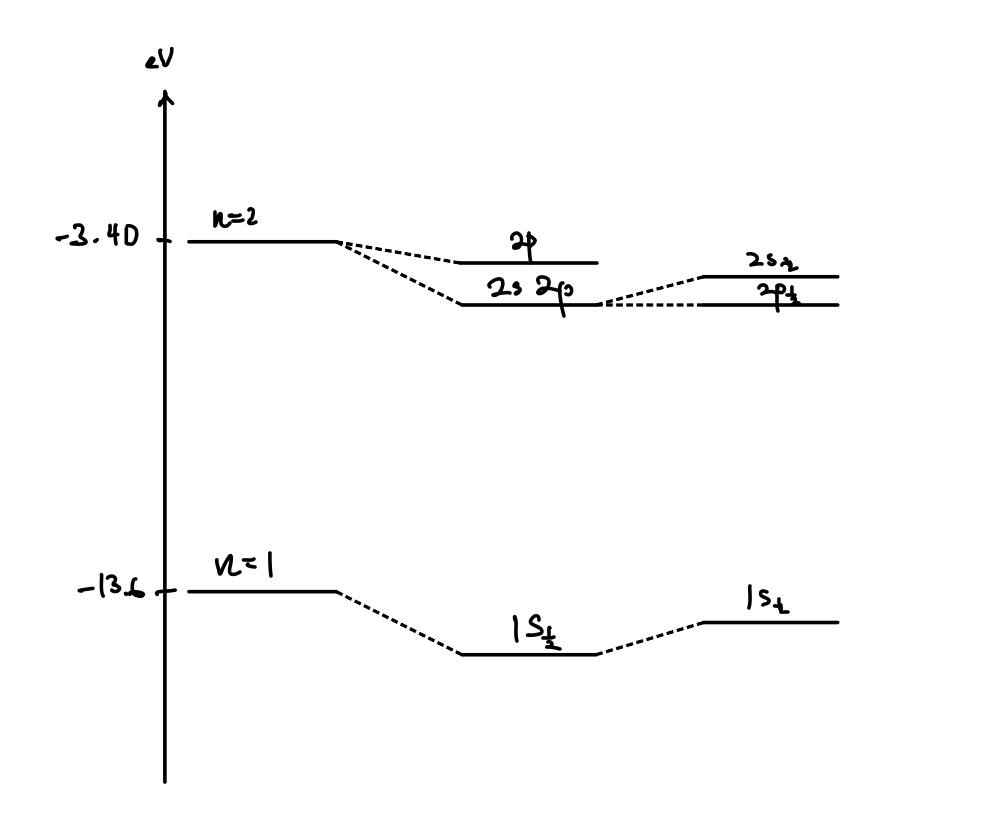
\includegraphics[width=5in]{./image/EnergyLevel.jpg}
        \caption{The energy level of Hydrogen Atom}
      \end{figure}

    The scales of the corrections attributed to the fine structure and the 
    Lamb shift are proportional to the fourth and fifth powers of the fine-structure constant, 
    $\alpha$, respectively.  

    \newpage
    \subsection{Fine structure functional form}
    The fine structure energy interval is given by:

    \begin{equation}
        \Delta E_{n,j} = \Delta E_{n,l}^{(0)} + \Delta E_{n,l}^{(1)} + \Delta E_{n,l}^{(2)}
    \end{equation}

    Subsituting the expression of $\Delta E_{n,l}^{(0)}$, $\Delta E_{n,l}^{(1)}$ and $\Delta E_{n,l}^{(2)}$ and simplify, we have:

    \begin{equation}
        \Delta E_{n,j} = -R^*_y Z^2 \left( \frac{Z^2 \alpha^2}{n^3 (j + \frac{1}{2})} - \frac{3 Z^2 \alpha^2}{4n^3}\right)
    \end{equation}

    From the above expression, we can arrange the terms to get the functional form of the fine structure energy interval:

    \begin{equation}
        \Delta E_{n,j} \approx \frac{1}{4n^3} + \frac{1}{4n^3} \propto \frac{1}{n^3}
    \end{equation}

    Therefore, the interval scales with $\frac{1}{n^3}$ and it is independent of the quantum number $l$.

    \subsection{Lamb Shift experime}

    The Lamb shift can be quantified using both Lamb Microwave Spectroscopy and Laser Spectroscopy, with each method 
    stimulating electron transitions across different energy levels. Laser Spectroscopy stands out for its greater 
    precision, attributed to its tighter linewidth and thus higher resolution in comparison to microwave techniques. 
    Furthermore, Laser Spectroscopy can employ Doppler-free saturated spectroscopy methods to counteract Doppler broadening 
    effects. On the other hand, in Microwave Spectroscopy, Doppler broadening has a more pronounced impact due to the diverse 
    velocities of the electrons relative to the microwave radiation source

    % Add a bibliography block to the postdoc
    
    
    
\end{document}
